\documentclass[letterpaper,final,12pt,reqno]{amsart}

\usepackage[total={6.3in,9.2in},top=1.1in,left=1.1in]{geometry}

\usepackage{times,bm,bbm,empheq,fancyvrb,graphicx}
\usepackage[dvipsnames]{xcolor}
\usepackage{longtable}
\usepackage{booktabs}

\usepackage[within=section]{newfloat}

\usepackage{tikz}
\usetikzlibrary{decorations.pathreplacing}

\usepackage[kw]{pseudo}
\pseudoset{left-margin=15mm,topsep=5mm,idfont=\texttt}

% hyperref should be the last package we load
\usepackage[pdftex,
colorlinks=true,
plainpages=false, % only if colorlinks=true
linkcolor=blue,   % ...
citecolor=Red,    % ...
urlcolor=black    % ...
]{hyperref}

\renewcommand{\baselinestretch}{1.05}

\allowdisplaybreaks[1]  % allow display breaks in align environments, if they avoid major underfulls

\newtheoremstyle{claim}% name
  {5pt}% space above
  {5pt}% space below
  {\itshape}% body font
  {}% indent amount
  {\itshape}% theorem head font
  {.}% punctuation after theorem head
  {.5em}% space after theorem head
  {\thmname{#1}\thmnumber{ #2}\thmnote{ (#3)}}% theorem head spec
\theoremstyle{claim}
\newtheorem{theorem}{Theorem}
\newtheorem{lemma}{Lemma}

\newcommand{\eps}{\epsilon}
\newcommand{\RR}{\mathbb{R}}

\newcommand{\grad}{\nabla}
\newcommand{\Div}{\nabla\cdot}
\newcommand{\trace}{\operatorname{tr}}

\newcommand{\hbn}{\hat{\mathbf{n}}}

\newcommand{\bb}{\mathbf{b}}
\newcommand{\be}{\mathbf{e}}
\newcommand{\bbf}{\mathbf{f}}
\newcommand{\bg}{\mathbf{g}}
\newcommand{\bn}{\mathbf{n}}
\newcommand{\br}{\mathbf{r}}
\newcommand{\bu}{\mathbf{u}}
\newcommand{\bv}{\mathbf{v}}
\newcommand{\bw}{\mathbf{w}}
\newcommand{\bx}{\mathbf{x}}

\newcommand{\bF}{\mathbf{F}}
\newcommand{\bV}{\mathbf{V}}
\newcommand{\bX}{\mathbf{X}}

\newcommand{\bxi}{\bm{\xi}}

\newcommand{\bzero}{\bm{0}}

\newcommand{\rhoi}{\rho_{\text{i}}}

\newcommand{\ip}[2]{\left(#1,#2\right)}

\newcommand{\mR}{R^{\bm{\oplus}}}
\newcommand{\iR}{R^{\bullet}}

\newcommand{\nn}{{\text{n}}}
\newcommand{\pp}{{\text{p}}}
\newcommand{\qq}{{\text{q}}}
\newcommand{\rr}{{\text{r}}}

\newcommand{\bus}{\bu|_s}

% norm |||x|||
\newcommand{\vertiii}[1]{{\left\vert\kern-0.25ex\left\vert\kern-0.25ex\left\vert #1 \right\vert\kern-0.25ex\right\vert\kern-0.25ex\right\vert}}

% numbering
\setcounter{tocdepth}{3}
\makeatletter
\def\l@subsection{\@tocline{2}{0pt}{4pc}{5pc}{}}
\makeatother

\numberwithin{equation}{section}
\numberwithin{figure}{section}
\numberwithin{table}{section}
\numberwithin{theorem}{section}

\DeclareFloatingEnvironment[name=Pseudocode]{pcode}

\begin{document}
\title[Multilevel computation of glacier geometry from Stokes dynamics]{Multilevel computation of glacier geometry \\ from Stokes dynamics}

\author{Ed Bueler}

\author{Lawrence Mitchell}

\date{\today}

\begin{abstract} FIXME MCD for steady and evolving geometry with Glen-Stokes dynamics
\end{abstract}

\maketitle

%\tableofcontents

\thispagestyle{empty}
%\bigskip

\section{Introduction} \label{sec:intro}

FIXME a multigrid \cite{Trottenbergetal2001} method basically by \cite{Tai2003} for obstacle problems; see \cite{Bueler2022} and \cite{GraeserKornhuber2009};  obstacle problem view first extended to Stokes by \cite{WirbelJarosch2020}


\section{The steady ice geometry problem} \label{sec:stokesgeometry}

The standard model for determining the geometry of glaciers is based upon a dynamical description of ice flow, namely a shear-thinning version of the Stokes equations.  However, this Glen-Stokes ice-dynamics model only determines the free-surface glacier geometry when combined with the surface kinematical equation (SKE) and a climate input, namely the balance of the rates of snow accumulation and melting/runoff (ablation).  In this section we state the strong form of the resulting ``coupled'' glacier geometry model in the steady-state case, which we call the steady ice geometry problem (SIGP).  The emphasis here is on the complementarity-problem nature of the SIGP, which is often not explicit in the glaciers literature (but see \cite{SchoofHewitt2013}).  We then define the weak form, noting along the way several unresolved aspects of the theory.  The steady model has a straightforward extension to a time-discretized evolving-geometry model, the implicit ice geometry problem (IIGP; Section \ref{sec:evolution}).

The SIGP is defined on a fixed, bounded map-plane region $\Omega \subset \RR^d$ for $d=1,2$ (Figure \ref{fig:stokesdomain}; coordinates on $\Omega$ are denoted as $x$ when $d=1$ and $x,y$ when $d=2$).  On $\Omega$ we assume that a time-independent climatic mass balance (CMB) \cite{Cogleyetal2011} function $a(x,y)$ is defined at every point, whether or not ice is present at that location.  In ice-free areas this function is the ``potential'' CMB, namely the annual balance of snow accumulation and melt if ice were present, e.g.~as computed by energy balance in a climate or weather model.  We assume $a$ has units of ice thickness per time, compatible with our assumption of constant ice density.  Also, a bed elevation function $b(x,y)$ is defined everywhere on $\Omega$; it gives the topography upon which the glacier sits.  The functions $a$ and $b$ are the data (inputs) of the SIGP.

\begin{figure}[t]
\begin{center}
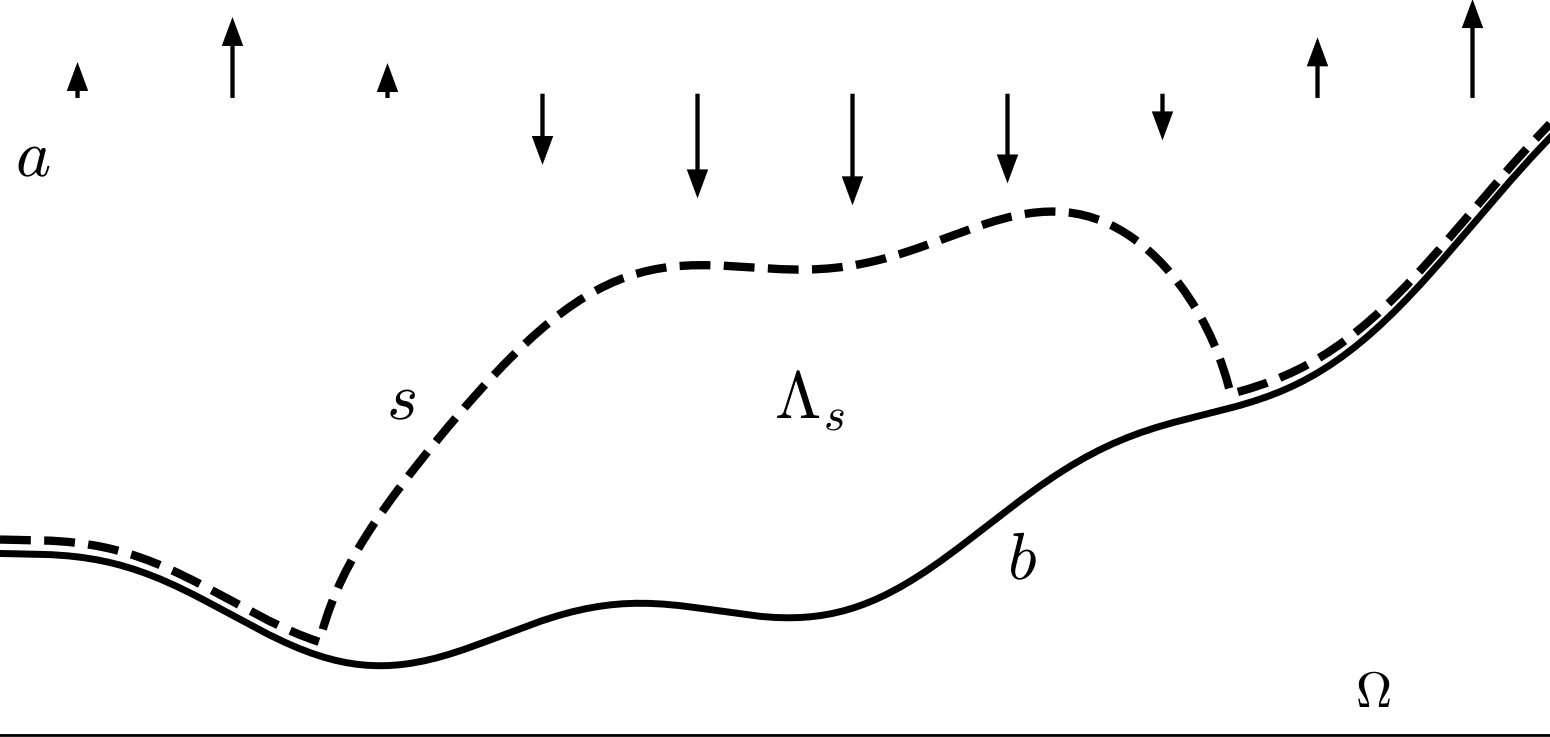
\includegraphics[width=0.7\textwidth]{genfigs/stokesdomain.pdf}
\end{center}
\caption{In the SIGP the CMB $a$ (arrows; down for accumulation) and bed elevation $b$ (solid) are given data on a map-plane region $\Omega \subset \RR^d$ for $d=1,2$.  The solution includes a surface elevation $s$ (dashed) on $\Omega$, such that $s\ge b$, plus the ice velocity $\bu$ and pressure $p$ on the icy domain $\Lambda_s = \{b < z < s\} \subset \RR^{d+1}$.}
\label{fig:stokesdomain}
\end{figure}

Now, the Glen-Stokes stress balance equations (below) only apply in a certain icy domain in $\RR^{d+1}$.  We make a strong, but common \cite[for example]{IsaacStadlerGhattas2015,Jouvetetal2008,Lengetal2012,WirbelJarosch2020} assumption that this domain has a well-defined upper surface elevation, a function $s(x,y)$.  That is, we assume there are \emph{no overhangs}, and that the under-side of the ice is in contact with the bed $b$.  We then define $s$ everywhere in $\Omega$ by extending with $s=b$ where ice is absent, thus $s\ge b$ applies on all of $\Omega$.  Note that $s$ is part of the model solution; it is not given data.

Based on this well-defined upper surface, the icy domain is the open set
\begin{equation}
\Lambda_s = \{(x,y,z)\,|\,(x,y) \in \Omega \,\text{ and }\, b(x,y) < z < s(x,y)\}  \subset \RR^{d+1}, \label{eq:lambdas}
\end{equation}
where $z$ is vertically-upward.  The domain $\Lambda_s$, which is a \emph{solution} in our model, has the topology of the product of an open subset of $\Omega$ and an interval, and we will approximate it using an extruded mesh (Section \ref{sec:fe}).

We model the ice as an incompressible, very-viscous \cite{Acheson1990}, non-Newtonian fluid in $\Lambda_s$.  Allowing any Glen exponent $\nn\ge 1$ \cite{GreveBlatter2009}, the equations are
\begin{align}
- \nabla \cdot \tau + \nabla p &= \rhoi \bg &&\text{\emph{stress balance}} \label{eq:forcebalance} \\
\nabla \cdot \bu &= 0 &&\text{\emph{incompressibility}} \label{eq:incompressible} \\
\tau &= B_\nn |D\bu|^{(1/\nn) - 1} D\bu  &&\text{\emph{flow law}} \label{eq:viscflowlaw}
\end{align}
The solution fields here are the velocity $\bu$, pressure $p$, and deviatoric stress $\tau$.  Equations \eqref{eq:forcebalance} and \eqref{eq:viscflowlaw} form the momentum conservation (stress balance) model, while \eqref{eq:incompressible} follows from constant density and mass conservation \cite[Chapter 1]{FowlerNg2021}.

Regarding tensors and their notation, recall that the Cauchy stress tensor $\sigma$ decomposes into the deviatoric part $\tau$ minus the pressure, i.e.~$\sigma = \tau - p\,I$, so equation \eqref{eq:forcebalance} simply says $-\Div \sigma = \rhoi \bg$.  The strain rate tensor $D\bu$ is the symmetric part of $\grad \bu$, $D\bu = \frac{1}{2} \left(\grad\bu + \grad\bu^\top\right)$, and the tensor norm used in \eqref{eq:viscflowlaw} satisfies $|D\bu|^2 = \frac{1}{2} (D\bu)_{ij} (D\bu)_{ij}$.  Because $D\bu$ is symmetric, and because it has trace zero by equation \eqref{eq:incompressible}, i.e.~$\trace(D\bu)=\nabla \cdot \bu = 0$, equation \eqref{eq:viscflowlaw} then implies that $\tau$ is also symmetric with trace zero, thus that $p=-\trace \sigma / (d+1)$.

In computations we will use the following constants: Glen exponent $\nn=3$, ice density $\rhoi=910 \,\text{kg}\,\text{m}^{-3}$ \cite{Huybrechtsetal1996}, and gravity $\bg=\left<0,0,-g\right>$, with $g=9.81\,\text{m}\,\text{s}^{-2}$.  The ice hardness $B_\nn$ is a constant because we assume isothermal conditions \cite{GreveBlatter2009}, with value $B_3=6.8082\times 10^7\,\text{Pa}\,\text{s}^{1/3}$ \cite{Huybrechtsetal1996}.

For the $\nn=1$ (Newtonian) Stokes equations one would write \eqref{eq:viscflowlaw} as $\tau = 2\nu D\bu$ with viscosity $\nu>0$, but exponents $\nn>1$ suggest an effective viscosity function of $|D\bu|$.  This would be singular in the limit of small strain rates, and so, motivated by the actual finite viscosity of glacier ice \cite{GreveBlatter2009}, we define the following regularized effective viscosity using $\eps>0$,
\begin{equation}
\nu_\eps(|D\bu|) = \frac{1}{2} B_\nn \left(|D\bu|^2 + \eps\, D_0^2\right)^{(\pp-2)/2}, \label{eq:regeffvisc}
\end{equation}
where $\pp=(1/\nn)+1$, with $\pp=4/3$ in computations.  The constant $D_0$ defines a strain-rate scale for glacier flow; values $D_0 = 1 \,\text{a}^{-1}$ and $\eps = 10^{-4}$ are used in computations.

Our SIGP model uses dynamic boundary conditions for an isolated, grounded, and non-sliding glaciers.  (Floating and sliding cases are topics for additional research.)  In addition to the already-stated assumption that the top and bottom boundaries of $\Lambda_s$ can be identified, we further assume these surfaces have well-defined tangents.  On the base we impose no slip:
\begin{equation}
\bu = \bzero  \qquad\qquad \text{\emph{base} } \Gamma_0. \label{eq:basebc}
\end{equation}
On the sub-aerial surfaces we set a condition of zero applied stress,
\begin{equation}
\left(2 \nu_\eps(|D\bu|) D\bu - pI\right) \bn = \bzero  \qquad \qquad \text{\emph{upper ice surface}} \label{eq:topbc}
\end{equation}
where $\bn$ is any normal to $\partial \Lambda_s$.  (A nonzero atmospheric pressure at the surface is straightforward to apply if desired.)  Note that the ice flow extends in the horizontal direction until a free boundary at the glacier margin is reached.  Generally $\grad s$ is singular at a glacier margin.

The simultaneous determination of $\Lambda_s$ and $(\bu,p)$ is the goal of the SIGP model.  However, the above equations make no reference to the climate input function $a$, so we need another ``equation'', one which is fundamentally an inequality as well.  Noting that the surface elevation is already defined on all of $\Omega$, with $s=b$ off the ice, we set
\begin{equation}
\bn_s = \left<-s_x,-s_y,1\right> \label{eq:surfacenormal}
\end{equation}
as an (un-normalized) top-surface normal defined almost everywhere on $\Omega$.  Furthermore we extend the surface value of the velocity to all of $\Omega$:
\begin{equation}
\bus(x,y) = \begin{cases} \bu(x,y,s(x,y)), & s(x,y) > b(x,y), \\
                     \bzero, & \text{elsewhere}. \end{cases} \label{eq:surfacevelocity}
\end{equation}
A discontinuity of this function is (generally) expected at the ice margin.

The steady-state surface kinematical equation (SKE) \cite[equation (5.21)]{GreveBlatter2009} is the needed additional equation:
\begin{equation}
\bus \cdot \bn_s + a = 0 \qquad \text{\emph{on the ice}}. \label{eq:ske}
\end{equation}
Note that $a(x,y)$ is the \emph{vertical} ice thickness added per time \cite{GreveBlatter2009}.  Though kinematical balance \eqref{eq:ske} applies only on the ice, $\bus \cdot \bn_s + a \le 0$ applies everywhere in $\Omega$ because $a$ is nonpositive in steady state in ice-free locations.  In fact, when combined with the constraint that $s\ge b$ everywhere on $\Omega$, SKE \eqref{eq:ske} is part of an infinite-dimensional nonlinear complementarity problem (NCP) \cite{Bueler2021conservation}.  By definition, an NCP on a vector space $V$ combines the three statements
\begin{equation}
x\ge 0, \quad f(x)\ge 0, \quad x f(x)=0 \label{eq:ncp}
\end{equation}
for all $x\in V$, where $f:V\to V$ \cite{FacchineiPang2003}.

We may now state the strong form of the SIGP, as follows, by including all of the above conditions, and also by eliminating $\tau$ from \eqref{eq:forcebalance} and \eqref{eq:viscflowlaw}:
\begin{align}
s - b &\ge 0 && \text{on $\Omega$} \label{eq:strongform} \\
- \bu|_s \cdot \bn_s - a &\ge 0 && \text{\emph{same}} \notag \\
(s - b) (- \bu|_s \cdot \bn_s - a) &= 0 && \text{\emph{same}} \notag \\
- \nabla \cdot \left(2 \nu_\eps(|D\bu|)\, D\bu\right) + \nabla p - \rhoi \mathbf{g} &= \bzero && \text{on $\Lambda_s$} \notag \\
\nabla \cdot \bu &= 0 && \text{\emph{same}} \notag \\
\bu &= \bzero && \text{on $\Gamma_0$} \notag \\
\left(2 \nu_\eps(|D\bu|) D\bu - pI\right) \bn &= \bzero && \text{on $\partial \Lambda_s \setminus \Gamma_0$} \notag
\end{align}
The first three statements in \eqref{eq:strongform} form the NCP, but this problem is coupled to the boundary value problem formed by the last four statements.

The solution of \eqref{eq:strongform} is a triple of functions $s(x,y)$, $\bu(x,y,z)$, $p(x,y,z)$ on $\Omega,\Lambda_s,\Lambda_s$, respectively.  However, as the domain on which $\bu,p$ are defined is only known via the solution, \eqref{eq:strongform} is at best an incomplete description.  (The weak form in the next section, using a solution operator which maps $s$ to $\bu|_s$, will address this concern.)  However, whether in strong or weak form, inequality-constrained system \eqref{eq:strongform} has a largely-unresolved theory regarding well-posedness and solution regularity.  Certain well-posedness theory is known for the SIA version of this problem, with existence established by \cite{JouvetBueler2012}, including uniqueness in the flat bed case.

As a consequence of the no-overhangs assumption, the SIGP as described here is likely not to be well-posed because of an issue at the ice margin.  There may be no steady state because the fluid in the vicinity of a steep ice margin, especially on a steep bed feature, generates an overhang, violating the assumption that the function $s$ is well-defined.  Furthermore the same concern applies to each time step of an evolving model; overhangs can develop at the margin.  Because overhangs are small features in large glaciers and ice sheets, most modeling literature ignores this possibility and assumes well-defined surface elevation and thickness \cite{Jouvetetal2008,Lengetal2012,WirbelJarosch2020}.  The exceptional literature \cite{Jouvetetal2011,PralongFunk2005} provides a model in which ice-cliff calving occurs via a damage variable and a stress-fracture failure criterion, which might explain how a (nearly) well-defined surface elevation and thickness could arise in a more-complete, and well-posed, model.  However, such a model is a nontrivial extension of the above equations.  Neither marginal cliffs nor overhangs are allowed in our theory.

After stating the SIGP weak form next in Section \ref{sec:weakido}, in Sections \ref{sec:fe}--\ref{sec:results} we will construct and demonstrate a multilevel scheme for the problem.  Noting that numerical solutions have traditionally applied explicit time-stepping, even when computing steady states, splitting the dynamics and the SKE into sub-steps and using truncation to address the NCP \cite[for example]{Jouvetetal2008,Lengetal2012}, the implicit time-stepping model in Section \ref{sec:evolution} avoids time-splitting and is unconditionally stable.


\section{The weak form using an ice dynamics operator} \label{sec:weakido}

The weak form of the fixed-geometry Glen-Stokes model for ice flow, which extends the linear Stokes weak form \cite{Elmanetal2014} to regularized power-law rheology, is relatively well-known \cite{IsaacStadlerGhattas2015,JouvetRappaz2011,Lengetal2012}, and we summarize it here.  Then we address the weak form of the geometry-determining SIGP.

Denote by $W^{k,r}$ the Sobolev space \cite{Evans2010} of functions with $k$ weak derivatives which are $r$th-power integrable.  Suppose for the moment that $\Lambda \subset \RR^{d+1}$ is a fixed, bounded domain on which we prescribe a Dirchlet condition $\bu=0$ on some positive-measure portion of $\partial\Lambda$, and otherwise suppose the boundary is stress-free (Neumann boundary).  Let $\pp=(1/\nn)+1$ as in \eqref{eq:regeffvisc}, and $\qq=(1-\pp^{-1})^{-1}=\nn+1$ the conjugate exponent; $\pp=4/3$ and $\qq = 4$ if $\nn=3$.  Let $W_0^{1,\pp}(\Lambda)^{d+1}$ be the space of velocity functions, zero along the Dirichlet boundary, and let
\begin{equation}
\mathcal{M}_\Lambda = W_0^{1,\pp}(\Lambda)^{d+1} \times L^\qq(\Lambda)  \label{eq:mixed}
\end{equation}
be the (mixed) space of admissible velocity and pressure pairs.  The Glen-Stokes solution $(\bu,p) \in \mathcal{M}_\Lambda$ satisfies the weak form
\begin{equation}
F_\Lambda(\bu,p)[\bv,q] = \int_\Lambda 2 \nu_\eps(|D\bu|) D\bu : D\bv - p \Div\bv - (\Div\bu) q - \rhoi \bg \cdot \bv\,d\bx = 0 \label{eq:glenstokesweak}
\end{equation}
for all $(\bv,q) \in \mathcal{M}_\Lambda$.  If $\bu,p$ are sufficiently regular then they satisfy strong equations \eqref{eq:forcebalance}--\eqref{eq:topbc}.  Jouvet and Rappaz \cite{JouvetRappaz2011} prove that this fixed-domain Glen-Stokes formulation is well-posed under the above assumptions if also the Neumann boundary of $\Lambda$ is $C^1$.  They show \eqref{eq:glenstokesweak} is equivalent to minimization of a convex and coercive functional over the divergence-free subspace, and that there is a unique pressure $p$.

However, we must go beyond predetermined ice geometry to solve the weak form of SIGP \eqref{eq:strongform}.  Again suppose $\Omega \subset \RR^d$ is a fixed map-plane domain with $C^1$ boundary, and that the bed elevation $b$ is in $W^{1,\qq}(\Omega)$.  The Sobolev space $W^{1,\qq}(\Omega)$ supports a linear trace operator which defines the symbol $|_{\partial \Omega}$ \cite[Section 5.5]{Evans2010}.  Let
\begin{equation}
\mathcal{K} = \{s \in W^{1,\qq}(\Omega) \,:\, s \ge b \, \text{ and } \, s\big|_{\partial\Omega} = b\big|_{\partial\Omega}\}  \label{eq:Kconstraintset}
\end{equation}
be the closed and convex set of admissible surface elevations of an isolated glacier or ice sheet.  From now on we also assume that $\nn>1$.  Because $\qq = \nn+1 > d$, each $s \in W^{1,\qq}(\Omega)$ is continuous \cite[Morrey's inequality, section 5.6.2]{Evans2010}, and so there are no cliffs in the $s$ geometry.  (Though it is not yet clear that the correct Sobolev space is identified in \eqref{eq:Kconstraintset}, existence for the simpler SIA model finds that a power of the ice thickness, $u=(s-b)^{2q/(q-1)}$, is in $\mathcal{K} = \{v \ge 0\} \subset W^{1,\qq}(\Omega)$ \cite{JouvetBueler2012}.)  Recalling definition \eqref{eq:lambdas}, we further suppose that
\begin{equation}
s\in \mathcal{K} \text{ defines an icy domain } \Lambda_s \text{ which has a $C^1$ upper surface.} \label{eq:quixotic}
\end{equation}
Assumption \eqref{eq:quixotic} would follow from a sufficiently-strong regularity result for the theory of the current paper, something we cannot offer.  However, in the SIA model the surface $s$ solves an elliptic equation, and $s$ is $C^1$ on $\{s>b\} \subset \Omega$ if $b$ is continuous \cite{JouvetBueler2012}.

We now define an ice dynamics operator (IDO), a map $\Phi$ which uses the trace of the velocity solution to the Glen-Stokes problem \eqref{eq:glenstokesweak}; see Figure \ref{fig:idoaction}.  For each $s \in \mathcal{K}$ the output $\Phi(s)$ is the negative normal component of the (unique) velocity solution $\bu$ of \eqref{eq:glenstokesweak} over the upper surface of $\Lambda_s$, but extended by zero to all of $\Omega$:
\begin{equation}
\Phi(s) = \begin{cases} - \bu|_s \cdot \bn_s, & s > b, \\
                        0, & \text{otherwise}. \end{cases} \label{eq:ido}
\end{equation}
Here $\bu|_s$ denotes a trace operator on $W^{1,\pp}(\Lambda_s)^{d+1}$; compare \eqref{eq:mixed}.  Note that $\Phi(s)$ is a scalar function on $\Omega$ which may jump or be singular at the glacier margin even if $s$ is smooth on $\{s>b\}$.  We will only need $\Phi(s)$ to be in the dual of $W^{1,\qq}(\Omega)$.

\begin{figure}[t]
\begin{center}
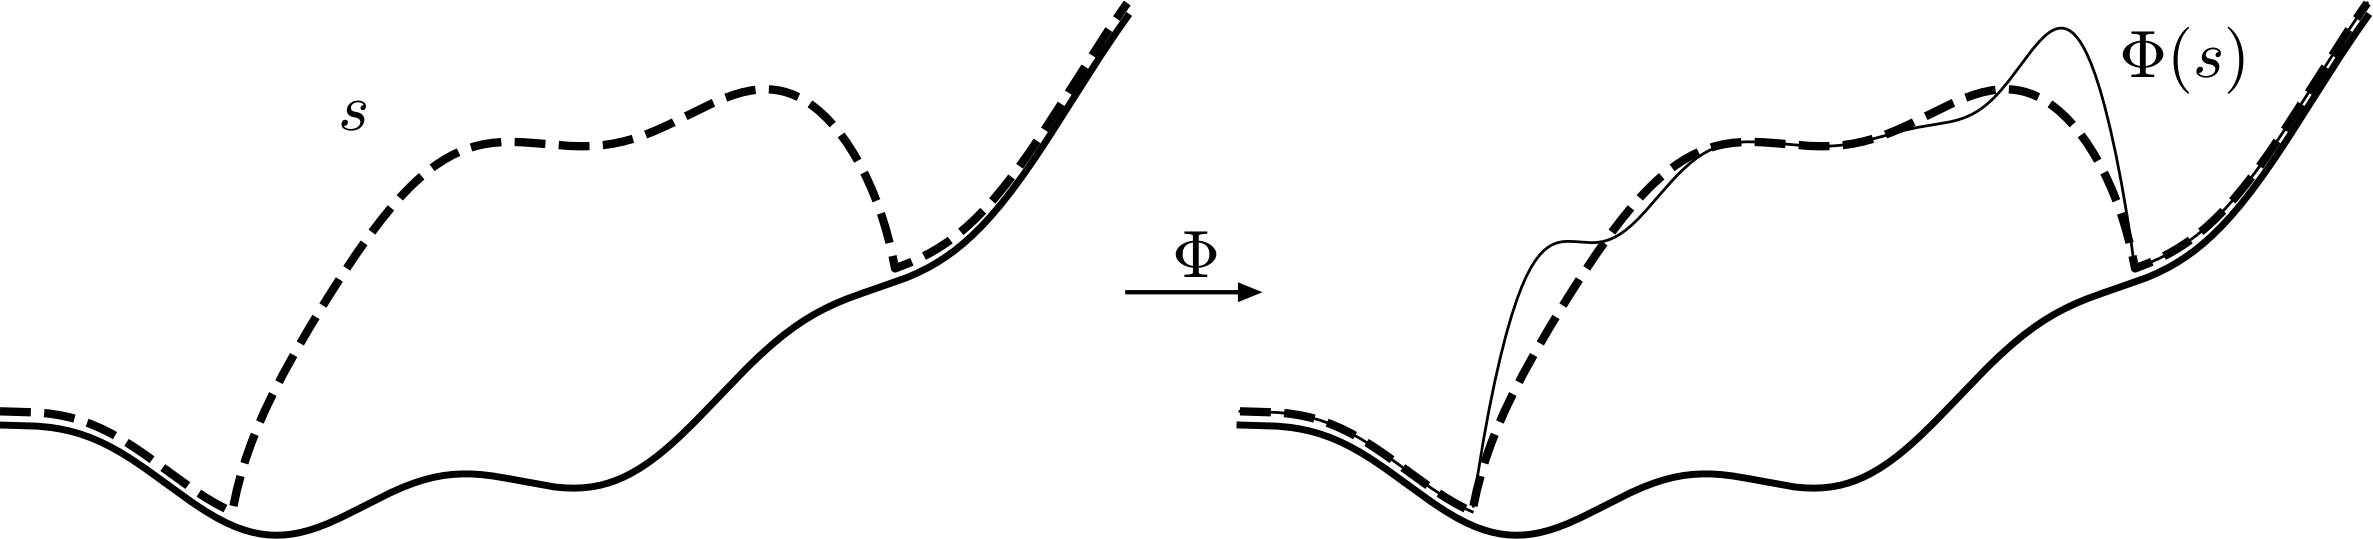
\includegraphics[width=\textwidth]{genfigs/idoaction.pdf}
\end{center}
\caption{The IDO $\Phi$ maps the surface elevation $s$ (dashed) to the normal ice surface motion $\Phi(s)=- \bu|_s \cdot \bn_s$.  Both $s$ and $\Phi(s)$ are defined on all of $\Omega$, but $\Phi(s)$ is generally discontinuous.}
\label{fig:idoaction}
\end{figure}

We believe that formula \eqref{eq:ido} defines a nonlinear operator $\Phi:\mathcal{K} \subset W^{1,\qq}(\Omega) \to (W^{1,\qq}(\Omega))^* = W^{-1,\pp}(\Omega)$.  This operator is \emph{expensive} and \emph{nonlocal}.  Evaluating $\Phi(s)$ requires solving Glen-Stokes problem \eqref{eq:glenstokesweak} on $\Lambda_s \subset \RR^{d+1}$ defined in \eqref{eq:lambdas}, and furthermore the solution $\bu$ is influenced everywhere by changes in the icy domain geometry.  In particular, if $\tilde s=s + r$ defines $\Lambda_{\tilde s} \supset \Lambda_s$, for $r\in C_c^\infty(\Omega)$ with $r\ge 0$ supported inside $\{s>b\}$, then the Stokes solutions are generically different \emph{everywhere}; generically $\tilde\bu - \bu \ne 0$ a.e.~on $\Lambda_s$.  It follows that an FE discretization (Section \ref{sec:fe}) of $\Phi(s)$ will have a dense Jacobian matrix.

By contrast, in the simpler isothermal, nonsliding, $d=2$ SIA model the operator is a nonlinear, second-order differential operator,
\begin{equation}
\Phi_{\text{SIA}}(s) = - \frac{\gamma}{\qq} (s-b)^{\qq} |\grad_2 s|^{\qq} - \grad_2 \cdot\left[\frac{\gamma}{\qq+1} (s-b)^{\qq+1} |\grad_2 s|^{\qq-2} \grad_2 s\right], \label{eq:phisia}
\end{equation}
for $\gamma = 2(\rhoi g)^{\nn} (B_\nn)^{-\nn} > 0$ constant and $\grad_2 = (\partial_x,\partial_y)$.  Thus an FE discretization of $\Phi_{\text{SIA}}(s)$ has sparse Jacobian.  However, $\Phi_{\text{SIA}} \approx \Phi$ for shallow glaciers to the degree that the lubrication approximation \cite{Acheson1990} is valid, and in fact for ice sheets we expect the Jacobian of $\Phi$ to be well-approximated by a banded matrix.

In this section we will use $\Phi$ to simplify the SIGP strong form and express its weak form, but later we will be concerned with two other aspects of the IDO:
\renewcommand{\labelenumi}{(\emph{\roman{enumi}})}
\begin{enumerate}
\item Section \ref{sec:smoothers} approximates the diagonal entries of the Jacobian $\Phi'$ to construct smoothers.
\item Section \ref{sec:evolution} relates the spectrum of $\Phi'$ to the stability of time-stepping methods.
\end{enumerate}

For now we re-write \eqref{eq:strongform} as a cleaner NCP with a hidden dynamical problem:
\begin{align}
s - b &\ge 0  \label{eq:idostrongform} \\
\Phi(s) - a &\ge 0 \notag \\
(s - b) (\Phi(s) - a) &= 0 \notag
\end{align}
These statements hold on all of $\Omega$, and the roles of the data $a,b$ are evident, and the solution is the ice surface $z=s(x,y)$, but the variables $\bu,p$ are hidden within the evaluation of $\Phi(s)$.

To reveal the SIGP weak form we define a functional which is simply the dual of $\Phi$:
\begin{equation}
F(s)[r] = \ip{\Phi(s)}{r} = \int_\Omega \Phi(s)\, r \,dx dy \label{eq:sigpfunctional}
\end{equation}
% in here one could integrate-by-parts on the vertical velocity using incompressibility:
% u|_s . n|_s = u|_s s_x + v|_s s_y + w|_s = u|_s s_x + v|_s s_y - \int_b^s (u_x + v_y) dz
% and then integrate by parts in plane
where $r \in W^{1,q}(\Omega)$.  One computes $F(s)[r]$ by defining $\Lambda_s$ as in \eqref{eq:lambdas}, solving \eqref{eq:glenstokesweak}, evaluating the surface trace of the velocity to compute $\Phi(s)$, and then integrating the result against (i.e.~dual pairing with) the test function $r$.  The weak form itself is the following variational inequality (VI) \cite{KinderlehrerStampacchia1980} for $s\in\mathcal{K}$:
\begin{equation}
F(s)[r - s] \ge \ip{a}{r-s} \quad \text{for all $r \in \mathcal{K}$.}  \label{eq:sigpweakform}
\end{equation}
One can prove that if $s$ is $C^1$ and solves \eqref{eq:sigpweakform} then it solves strong forms \eqref{eq:ske} and \eqref{eq:idostrongform} \cite{Bueler2021conservation}.  Note that the strong SKE \eqref{eq:ske}, which holds on $s>b$, is the interior condition of VI \eqref{eq:sigpweakform} \cite{KinderlehrerStampacchia1980}.

Speaking geometrically, \eqref{eq:sigpweakform} says that $s$ is located in $\mathcal{K}$, generically on $\partial\mathcal{K}$, at a point where $\Phi(s)-a$ points directly into $\mathcal{K}$.  (The ``angle'' between $\Phi(s)-a$ and an arbitrary vector $r-s$ pointing into $\mathcal{K}$ is at most $90^\circ$.)  It is well-known that certain VIs arise as inequality-constrained minimization problems \cite{GraeserKornhuber2009,KinderlehrerStampacchia1980}, but to the best of our knowledge \eqref{eq:sigpweakform} does \emph{not} arise in this way.  Existence has been proven for the SIA analog of VI \eqref{eq:sigpweakform} \cite{JouvetBueler2012}, and this SIA model is not a minimization except in the flat-bed case.

The SIGP weak form \eqref{eq:sigpweakform} is coupled to the Glen-Stokes weak form \eqref{eq:glenstokesweak} through definition \eqref{eq:ido} of the IDO $\Phi$.  VI problem \eqref{eq:sigpweakform} therefore has three fundamental nonlinearities:
\renewcommand{\labelenumi}{(\emph{\roman{enumi}})}
\begin{enumerate}
\item the Glen power-law rheology,
\item the inequality constraint, and
\item the nonlinearity of free-surface flow as a function of the surface.
\end{enumerate}
Regarding (\emph{ii}), observe that the solution of the classical obstacle problem for the linear Laplacian operator is a nonlinear function of the data \cite{KinderlehrerStampacchia1980}.  For (\emph{iii}), note that a free-surface flow for Newtonian (linear) rheology produces a nonlinear equation for the flow thickness, e.g.~as expressed in the kinematic wave equation \cite{Ockendonetal2003}.

We will need the (Gateaux) derivative of $\Phi$.  Suppose $s\in \mathcal{K}$, $\eps>0$, and $t \in W_0^{1,\qq}(\Omega)$ is such that $s+\eps t \in \mathcal{K}$.  Then
\begin{equation}
\Phi'(s)[t] = - \lim_{\eps\to 0^+} \frac{\bu|_{s+\eps t} \cdot \bn_{s+\eps t} - \bus \cdot \bn_s}{\eps} \label{eq:idoderiv}
\end{equation}
on $\{s>b\}$.  However, $\Phi'(s)[t]$ is a one-sided directional derivative on $\{s=b\}$.  That is, $s+\eps t\ge b$ is required for all sufficiently-small $\eps>0$, thus $t\ge 0$, on the (active) set where $s=b$.  To simplify we define an $s$-independent set
\begin{equation}
\mathcal{W}_+ = \{t \in W_0^{1,\qq}(\Omega) \,:\, t(x,y) \ge 0\}. \label{eq:infdefectset}
\end{equation}
Then $\Phi'(s)[t]$ is well-defined on inputs $(s,t) \in \mathcal{K} \times \mathcal{W}_+$, and $F'(s)[t,r]=\int_\Omega \Phi'(s)[t] r$ is well-defined for $(s,t,r) \in \mathcal{K} \times \mathcal{W}_+ \times W^{1,\qq}(\Omega)$.

The difference in \eqref{eq:idoderiv} depends on the support of $t$:
\begin{equation}
\bu|_{s+\eps t} \cdot \bn_{s+\eps t} - \bus \cdot \bn_s = \begin{cases}
           (\bu|_{s+\eps t} - \bus) \cdot \bn_{s+\eps t} + \eps\, \bus \cdot \left<t_x,t_y,0\right>, & s > b \\
           \bu|_{s+\eps t} \cdot \bn_{s+\eps t}, & s=b, t > 0 \\
           0, & s=b, t = 0.
                 \end{cases} \label{eq:differencecases}
\end{equation}
Thus a necessary condition for differentiability of $\Phi$ is that $\bu|_{s+\eps t} \cdot \bn_{s+\eps t} = o(\eps)$ on the ice-free area $\{s=b\}$.  In physical terms, the ice motion part of the SKE \eqref{eq:ske} must vanish for shrinking ice masses on bare ground, a reasonable supposition if the ice cannot slide.

In the next three sections we will construct an iterative, multilevel finite element solver for SIGP weak form \eqref{eq:sigpweakform}.  Performance and stability concerns related to evaluating $\Phi'$ are addressed in Section \ref{sec:smoothers}.


\section{Finite element discretization} \label{sec:fe}

Assume $d=2$ and that $\Omega \subset \RR^d$ is polygonal with triangulation $\mathcal{T}$.  (If $d=1$ then $\mathcal{T}$ would denote an interval decomposition of $\Omega$.)  Based on low expected regularity at the ice margin, we will represent surface elevations $s\in \mathcal{K}$ using the $P_1$ finite element (FE) space
\begin{equation}
\mathcal{V}^h = \{s \in C^0(\Omega) : s|_T \text{ is linear if } T \in \mathcal{T}\} \subset W^{1,\qq}(\Omega).
\end{equation}
Note \cite{JouvetBueler2012} makes the same FE choice for the corresponding SIA problem, and that, because of low regularity at the free boundary, $P_1$ is a common choice even for the classical obstacle problem with smooth data \cite{GraeserKornhuber2009}.

Let $b^h \in \mathcal{V}^h$ be the discretized bed elevation, e.g.~the $\mathcal{V}^h$ interpolant of $b$, and define the following closed and convex admissible subset of $\mathcal{V}^h$:
\begin{equation}
\mathcal{K}^h = \{s^h \in \mathcal{V}^h \,:\, s^h \ge b^h \text{ and } s^h|_{\partial\Omega} = b^h|_{\partial\Omega}\}.  \label{eq:feK}
\end{equation}
(Compare \eqref{eq:Kconstraintset}.)  Each $s^h\in \mathcal{K}^h$ defines a numerical icy domain $\Lambda_{s^h} \subset \RR^{d+1}$ as in \eqref{eq:lambdas}.  A triangle (interval) $T\in\mathcal{T}$ is said to be ice-free in $\Lambda_{s^h}$ if $s^h=b^h$ at every vertex of $T$, and icy otherwise.

Given $b^h \in \mathcal{V}^h$ and $s^h \in \mathcal{K}^h$, we use Firedrake to construct an extruded mesh \cite{McRaeetal2016} on $\Lambda_{s^h}$ consisting of triangular prisms (or quadrilaterals if $d=1$); the triangulation $\mathcal{T}$ of $\Omega$ is now called the ``base mesh''.  As shown in Figure \ref{fig:extruded}, each icy $T \in \mathcal{T}$ generates a column of $m_z \ge 1$ prism (quadrilateral) elements in the extruded mesh.  However, ice-free $T$ have no extruded mesh elements at all; these columns are empty.  The extruded mesh is regenerated each time $F^h(s^h)$ is evaluated, but the base mesh $\mathcal{T}$ is unchanged.

\begin{figure}[t]
\begin{center}
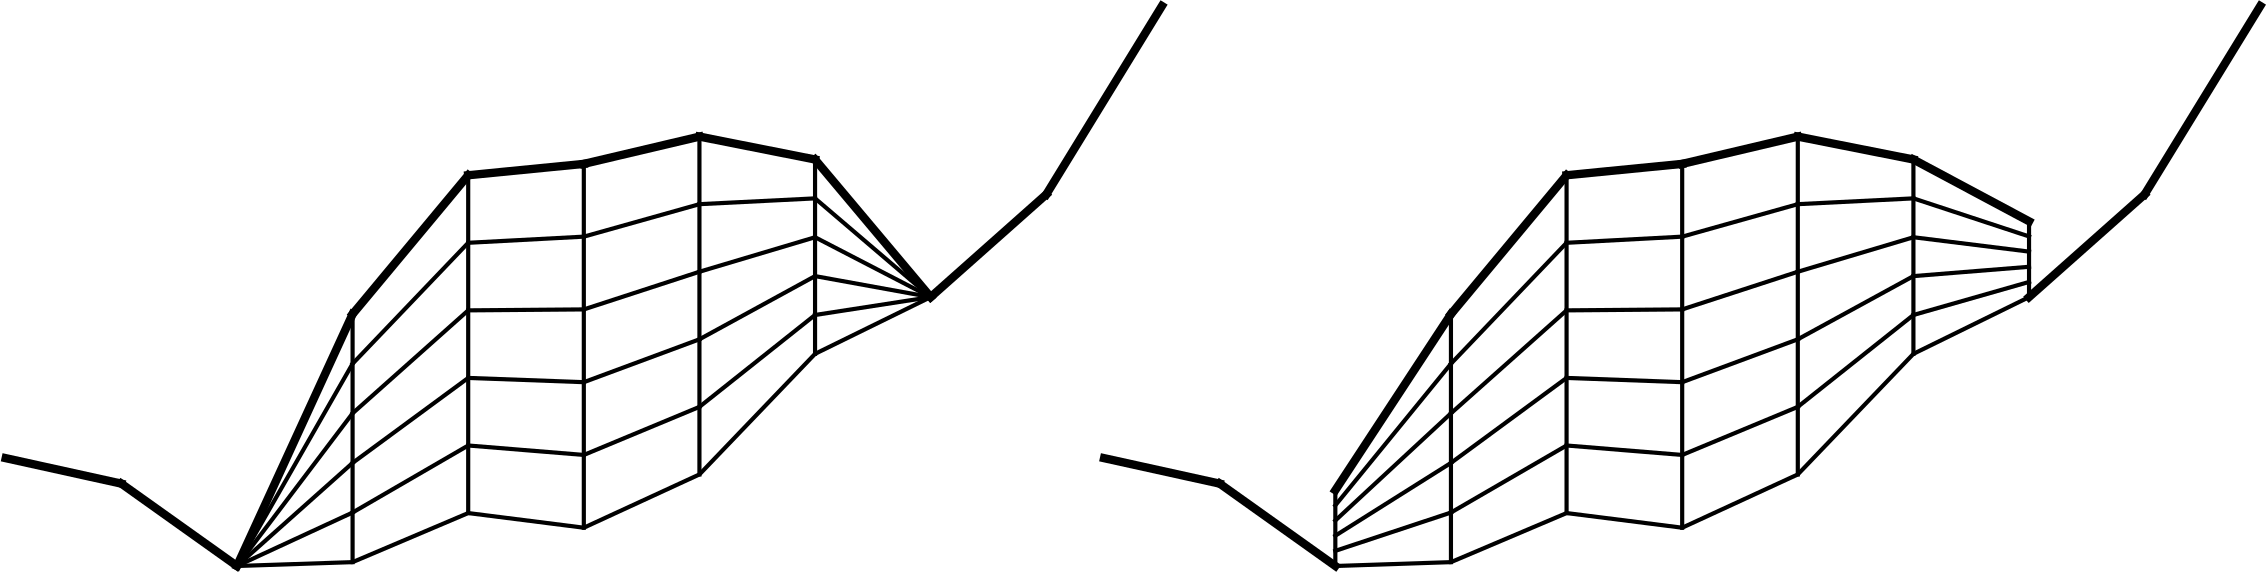
\includegraphics[width=\textwidth]{genfigs/extruded.pdf}
\end{center}
\caption{We compute the FE IDO $\Phi^h(s^h)$ by solving \eqref{eq:glenstokesweak} on an extruded mesh with $m_z$ layers.  In the ``pinched'' extrusion (left), the trace of $\bu^h$ is evaluated on the graph of $s^h$ (bold).  In the ``cliffs'' extrusion (right) all elements have a minimum thickness (dotted).}
\label{fig:extruded}
\end{figure}

On the extruded mesh we approximately solve Glen-Stokes problem \eqref{eq:glenstokesweak} using the $P_2\times P_1$ Taylor-Hood mixed space \cite{Elmanetal2014} which we denote $\mathcal{M}^h$.  Thus $(\bu^h,p^h) \in \mathcal{M}^h$ solves
\begin{align}
G_{\Lambda_{s^h}}(\bu^h,p^h)[\bv^h,q^h] &= 0  \label{eq:feglenstokesweak}
\end{align}
for all $(\bv^h,q^h) \in \mathcal{M}^h$, where
\begin{equation}
G_{\Lambda_{s^h}} = \int_{\Lambda_{s^h}} 2 \nu_\eps(|D\bu^h|) D\bu^h : D\bv^h - p^h \Div\bv^h - (\Div\bu^h) q^h - \rhoi \bg \cdot \bv^h\,d\bx.  \label{eq:feglenstokesfunctional}
\end{equation}

The power-law nonlinearity in \eqref{eq:feglenstokesweak} is resolved by using a Newton iteration, with direct solution of the step equations and back-tracking line search.  As stated in Section \ref{sec:intro}, our goal in the current paper is to show that $O(1)$ iterations of the multilevel scheme are needed to solve the discrete SIGP, \eqref{eq:fesigpweakform} below.  Overall optimality of the solution algorithm would also require an optimal solution of Glen-Stokes problem \eqref{eq:feglenstokesweak}, such as the multigrid scheme in \cite{IsaacStadlerGhattas2015}.

In fact we will compare two extrusion modes when solving problem \eqref{eq:feglenstokesweak}.  In the ``pinched'' extrusion the prism elements tile $\Lambda_{s^h}$ exactly but the elements at the ice margin are degenerate; they have positive volume but zero height at some nodes or even empty (vertical) facets.  In the alternate ``cliffs'' extrusion, each extruded element is nondegenerate and they tile a larger domain $\tilde\Lambda_{s^h} \supset \Lambda_{s^h}$.  Specifically, each prism has minimum thickness $H_{\text{min}}/m_z$ where $H_{\text{min}} > 0$ is the minimum total thickness, with $H_{\text{min}} = 20$ meters in computations.  The surface $s^h$ remains unchanged (and continuous), and cliffs only appear in problem \eqref{eq:feglenstokesweak}.

Let $\Phi^h:\mathcal{K}^h \to (\mathcal{V}^h)'$ be the FE approximation of the IDO $\Phi$.  By definition $\Phi^h(s^h)$ is the normal component of the numerical surface velocity after solving the Glen-Stokes equation \eqref{eq:feglenstokesweak} on the domain $\Lambda_{s^h}$.  That is, we evaluate $\Phi^h(s^h)$ using the surface trace as in \eqref{eq:ido}, and then extend by zero to all of $\Omega$.  In the ``cliffs'' extrusion the velocity trace is computed at the top of each column, and thus only nearby the original surface $s^h$, but the normal direction uses $s^h$ itself.

Finally, let $F^h(s)[r] = - \ip{\Phi^h(s)}{r}$; compare \eqref{eq:sigpfunctional}.  The discrete SIGP computes $s^h \in \mathcal{K}^h$ satisfying
\begin{equation}
F^h(s^h)[r^h - s^h] \ge \ip{a}{r^h-s^h} \quad \text{for all } r^h \in \mathcal{K}^h. \label{eq:fesigpweakform}
\end{equation}
The only role of the extruded mesh in solving \eqref{eq:fesigpweakform} is in the evaluation of the IDO $\Phi^h(s^h)$.  We believe that \eqref{eq:fesigpweakform} is well-posed in each extrusion mode, but we have no proof.


\section{Smoothers} \label{sec:smoothers}

In this section we consider single-level solvers for \eqref{eq:fesigpweakform}, namely certain nonlinear iterations which are made suitable for VIs \cite{KinderlehrerStampacchia1980}.  While these iterations are, in some cases, adequate smoothers in a multilevel method (next section), they converge slowly if used directly as solvers.  Because of the non-locality and density of the IDO $\Phi^h$ (Section \ref{sec:weakido}), we must make careful approximations in order to retain adequate per-iteration performance.  These iterative solvers, \emph{smoothers} from now on, can be categorized by the number of nodes which are adjusted at each iteration: pointwise, patch-type, and global.

Suppose there are $m$ interior vertices ($P_1$ nodes) of $\mathcal{T}$, denote a vertex in $\mathcal{T}$ by $(x_j,y_j)$, and let $\psi_j \in \mathcal{V}^h$ be the corresponding $P_1$ hat function, with $\psi_j(x_k,y_k)=\delta_{jk}$.  Let $s^h\in \mathcal{K}^h$ be the current surface elevation iterate.  The Richardson pointwise smoother sweeps through the nodes and subtracts-off the residual: $s^h \gets s^h - \alpha (F^h(s^h)-a)$ where $\alpha>0$ must be chosen so that the iteration converges.  By contrast the Gauss-Seidel, and Jacobi pointwise smoothers sweep through the nodes solving one-dimensional VI problems for a value $c\in \RR$ (below).  If each pointwise update $s^h \gets s^h + c \psi_i$ is done immediately then the smoother is of Gauss-Seidel (GS) type, also called serial or multiplicative, while a (parallel, additive) Jacobi smoother computes and stores solutions $c$ at every node before doing any updates.  In linear problems GS generally converges in about half as many iterations \cite{Greenbaum1997}.

To be more precise, let $\mathcal{W}_+^h = \{t^h \in \mathcal{V}^h \,:\, t^h \ge 0 \text{ and } t^h|_{\partial\Omega} = 0\}$.  If $i=0,\dots,m-1$ index the interior vertices of $\mathcal{T}$, note that $\psi_i \in \mathcal{W}_+^h$, and that $s^h + c \psi_i \in \mathcal{K}^h$ if and only if $c\ge \beta_i^{s^h} = b^h(x_i,y_i) - s^h(x_i,y_i)$.  (One might call $\beta_i^{s^h}$ the pointwise defect obstacle \cite{GraeserKornhuber2009} for $s^h$.)  The one-dimensional VI at interior node $i$ is derived from the discrete SIGP \eqref{eq:fesigpweakform} by replacements $s^h \to s^h+c \psi_i$, $r^h \to r^h + \gamma \psi_i$ for some scalars $c,\gamma$.  We then seek $c \ge \beta_i^{s^h}$ such that
\begin{equation}
F^h(s^h+c \psi_i)[(s^h+\gamma \psi_i) - (s^h+c \psi_i)] \ge \ip{a}{(s^h+\gamma \psi_i) - (s^h+c \psi_i)} \label{eq:fepointwiseviEARLY}
\end{equation}
for all $\gamma \ge \beta_i^{s^h}$.  Let
\begin{equation}
\rho_i(s^h; c) = F^h(s^h+c\psi_i)[\psi_i] - \ip{a}{\psi_i} \label{eq:ferhoi}
\end{equation}
be the pointwise residual function, and observe that \eqref{eq:fepointwiseviEARLY} simplifies to
\begin{equation}
(\gamma - c) \,\rho_i(s^h; c) \ge 0. \label{eq:fepointwisevi}
\end{equation}
The smoother approximately solves \eqref{eq:fepointwisevi} for $c$ and then updates $s^h \gets s^h + c \psi_i$ either in serial or parallel.  Observe that admissibility is preserved because $s^h+c \psi_i \in \mathcal{K}^h$ when $c \ge \beta_i^{s^h}$.

If $\rho_i(s^h; c)$ were linear and increasing in $c$, e.g.~$\rho_i(s^h; c) = \rho_i(s^h; 0) + \alpha c$ with $\alpha > 0$, then the solution to VI \eqref{eq:fepointwisevi} would be given by the simple formula $c = \max\left\{-\rho_i(s^h; 0)/\alpha, \beta_i^{s^h}\right\}$ \cite{GraeserKornhuber2009}.  In fact $\rho_i(s^h; c)$ is nonlinear, and we will linearize
\begin{equation}
\rho_i(s^h; c) \approx \rho_i(s^h; 0) + c\, \rho_i'(s^h; 0). \label{eq:rhoapprox}
\end{equation}
At each node where $\rho_i'(s^h; 0) > 0$ we will do one projected Newton step using the simple formula.  However, if $\rho_i'(s^h; 0) \le 0$, so that the model has degenerated in the sense that the linearized, pointwise operator is not acting elliptically with respect to a perturbation, we set $c = \beta_i^{s^h}$ to remove the ice at that location.  % FIXME TOO AGGRESSIVE?

Using a single Newton step and approximation \eqref{eq:rhofd}, GS is a well-defined smoother, so we state it in Pseudocode \ref{pc:pngsslow}.  It is given in a form which also allows over-relaxation ($\id{omega} > 1$) or under-relaxation ($\id{omega} < 1$) if desired.  Note that the Glen-Stokes problem \eqref{eq:glenstokesweak} is solved $2m$ times per application of this function.

\begin{pcode}[ht]
\begin{pseudo*}
\pr{pngs}(s^h,b^h,\id{omega}=1.0)\text{:} \\+
    \ct{check admissibility: $s^h \ge b^h$} \\
    for $i = 0,\dots,m-1$ \\+
        $\alpha_i = \rho_i'(s^h; 0)$  \qquad\qquad \ct{Jacobian diagonal entry} \\
        if $\alpha_i > 0$ \\+
            $c_i = - \rho_i(s^h; 0) / \alpha_i$ \\
            $(s^h)_i \gets \max\{(s^h)_i + \id{omega}\,c_i, (b^h)_i\}$ \\-
        else \\+
            $(s^h)_i \gets \beta_i$ \qquad\qquad \ct{non-elliptic case}
\end{pseudo*}
\caption{Projected nonlinear GS iteration, a conceptual in-place, pointwise smoother which solves one-dimensional VIs \eqref{eq:fepointwisevi} in serial.}
\label{pc:pngsslow}
\end{pcode}

Patch-type smoothers \cite{Farrelletal2021} have to our knowledge not been used for VI problems before, but they would sweep through the nodes solving local VIs of small dimension $\ell>1$, and again there would be serial and parallel versions.  However, we first consider the opposite extreme from a pointwise smoother, namely a global smoother in which all the degrees of freedom are coupled together into an algebraic system.

FIXME reduced-space Newton solver using a banded Jacobian approximation


\section{Approximate Jacobians} \label{sec:jacobians}

The above pseudocodes assume the accessibility of the diagonal of the Jacobian (pointwise smoothers) or of arbitrary entries (Newton solver).

Because the interior PDE in the SIA is elliptic, it follows that $\rho_i'(s^h; 0) > 0$ on the icy part of $\Omega$ \cite{JouvetBueler2012}, but for the full Glen-Stokes model there is no such guarantee to our knowledge.  Note that the derivative $\rho_i'(s^h; 0)$, which is also a diagonal entry of the Jacobian of $F^h$, can be approximated by a finite difference,
\begin{equation}
\rho_i'(s^h; 0) = (F^h)'(s^h)[\psi_i,\psi_i] \approx \frac{\rho_i(s^h; \eps) - \rho_i(s^h; 0)}{\eps}.  \label{eq:rhofd}
\end{equation}
Literal use of \eqref{eq:rhofd} is very expensive because each value $\rho_i(s^h; \eps)$ requires a separate Glen-Stokes computation for the residual.

A glaring difference between the GS and Jacobi smoothers now dominates.  Namely, GS imposes the expense of far more residual evaluations.

FIXME finite-difference approximation using pseudo-coloring based on ice thicknesses or rather longitudinal coupling length \cite{KambEchelmeyer1986}

To build a better smoother we return to the computation of the Jacobian diagonal entry $\rho_i'(s^h; 0)$.  Suppose we partition the support of $\psi_i$ into where there is ice and not,
\begin{equation}
\theta_i = \{\psi_i > 0\} \cap \{s^h > b^h\}, \qquad {\hat\theta}_i = \{\psi_i > 0\} \setminus \theta_i.  \label{eq:thetasupport}
\end{equation}
Recall that $\bu|_{z}$ denotes the surface velocity of the solution to the Glen-Stokes problem \eqref{eq:glenstokesweak} on the domain $\Lambda_{z}$, using an extruded mesh (Section \ref{sec:fe}).  By \eqref{eq:idoderiv}, \eqref{eq:differencecases}, and \eqref{eq:ferhoi} we may compute
\begin{equation}
\rho_i(s^h; 0) = F^h(s^h)[\psi_i] - \ip{a}{\psi_i} = - \int_{\theta_i} (\bu|_{s^h} \cdot \bn_{s^h}- a)\, \psi_i  \label{eq:rhozero}
\end{equation}
and
\begin{align}
\rho_i'(s^h; 0) &= (F^h)'(s^h)[\psi_i,\psi_i]  \label{eq:rholocalderiv} \\
  &= - \int_{\theta_i} \lim_{\eps\to 0^+} \frac{(\bu|_{s^h+\eps\psi_i} - \bu|_{s^h}) \cdot \bn_{s^h+\eps\psi_i}}{\eps} \psi_i - \int_{{\hat\theta}_i} \lim_{\eps\to 0^+} \frac{\bu|_{s^h+\eps\psi_i} \cdot \bn_{s^h+\eps\psi_i}}{\eps} \psi_i.  \notag
\end{align}

Clearly, any smoother application, which is a sweep over all nodes in $\mathcal{T}$, will require at least one Glen-Stokes velocity solution, namely from solving \eqref{eq:glenstokesweak} on the geometry determined by the current surface elevation $s^h$.  Formulas \eqref{eq:rhozero} and \eqref{eq:rholocalderiv} as stated require a Stokes solution $\bu|_{s^h+\eps\psi_i}$ for each mesh node.

However, we may estimate the surface velocity for a such perturbed surface elevation, namely with a small ``bump'' $\eps\psi_i$, by replacing the geometrical bump with a local perturbation of the body force.  That is, we may perturb the gravitational load relative to the solution which gave $s^h$, but without changing the geometry.  The change to the nonlinearities in this Glen-Stokes problem should be small, and the most important change to the velocity and pressure fields from a small bump perturbation is through its weight.  We suppose that other effects, such as a perturbed normal direction on the surface, are significantly smaller.

FIXME Let us fix a current surface elevation $s^h$ and assume that problem \eqref{eq:glenstokesweak} for $\Lambda_{s^h}$ yields solution $\bu^h,p^h$ at the convergence of its (Newton) iteration.  Noting that we are using a stable mixed space for this Glen-Stokes problem (Section \ref{sec:fe}), the final step in the iteration can be regarded as providing the solution of a linear system
\begin{equation}
    \begin{bmatrix} A & B^\top \\
                    B & 0      \end{bmatrix}
    \begin{bmatrix} \bu^h \\ p^h \end{bmatrix}
    = \begin{bmatrix} \rhoi \bg \\ 0 \end{bmatrix}.  \label{eq:system}
\end{equation}
where we note that the matrix depends on $s^h$.  (Even the size of $K$ depends on $s^h$ because it is used to determine which $T\in\mathcal{T}$ get extruded icy columns.)  Also denote the perturbed problem, for surface $s^h + \eps \psi_i$, using an $\eps$ subscript.

We assert that the perturbed-geometry Glen-Stokes solution is approximated by re-using the unperturbed matrix but adding the mass of the bump $\eps \psi_i$ to the right-hand side:
\begin{equation}
\begin{bmatrix} A_\eps & B_\eps^\top \\
                B_\eps & 0      \end{bmatrix}
\begin{bmatrix} \bu_\eps^h \\ p_\eps^h \end{bmatrix}
    = \begin{bmatrix} \rhoi \bg \\ 0 \end{bmatrix}
\qquad \approx \qquad
\begin{bmatrix} A & B^\top \\
                B & 0      \end{bmatrix}
\begin{bmatrix} \bu_\eps^h \\ p_\eps^h \end{bmatrix}
    = \begin{bmatrix}  \rhoi (1 + \eps \tau_i)\bg  \\ 0 \end{bmatrix}.  \label{eq:systemmassanalogy}
\end{equation}
Here $\tau_i$ is a positive $P_1$ function on $\Lambda_{s^h}$, that is, on the extruded $d+1$-dimensional mesh, with support only at the top-surface node with base mesh index $i$, and with magnitude such that if $\eps=1$ meter then
\begin{equation}
  \int_{\Lambda_{s^h}} \tau_i\,dx\,dy\,dz = \int_\Omega \psi_i\,dx\,dy . \label{eq:massanalogy}
\end{equation}
In words, we approximate the Glen-Stokes solution $\bu_\eps^h,p_\eps^h$ for the perturbed geometry by re-using the same (i.e.~$s^h$) geometry but solving the final linear system using a right-hand-side perturbation of the equivalent mass to the geometry perturbation.  This is shown in Figure \ref{fig:massanalogy}.

\begin{figure}[t]
\begin{center}
FIXME %\includegraphics[width=\textwidth]{genfigs/massanalogy.pdf}
\end{center}
\caption{A sketch of the mass-perturbation approximation in equations \eqref{eq:systemmassanalogy} and \eqref{eq:massanalogy}.}
\label{fig:massanalogy}
\end{figure}

FIXME Pseudocode \ref{pc:pnj} for PNJ with bump approximation

\begin{pcode}[ht]
\begin{pseudo*}
\pr{pnj}(s^h,b^h,\id{omega}=1.0)\text{:} \\+
    \ct{check admissibility: $s^h \ge b^h$} \\
    evaluate $\{\rho_i(s^h; 0)\}_{i=0}^{m-1}$  \qquad\qquad \ct{and save the final Newton step linear system} \\
    for $i = 0,\dots,m-1$ \\+
        $\alpha_i = (A^{-1})_{ii}$  \qquad\qquad \ct{FIXME: give correct Jacobian diagonal entry} \\
        if $\alpha_i > 0$ \\+
            $c_i = - \rho_i(s^h; 0) / \alpha_i$ \\--
    for $i = 0,\dots,m-1$ \\+
        if $\alpha_i > 0$ \\+
            $(s^h)_i \gets \max\{(s^h)_i + \id{omega}\,c_i, (b^h)_i\}$ \\-
        else \\+
            $(s^h)_i \gets \beta_i$ \qquad\qquad \ct{non-elliptic case}
\end{pseudo*}
\caption{Projected nonlinear Jacobi smoother using a bump approximation for the Jacobian diagonal entry $\alpha_i$.  Problem \eqref{eq:glenstokesweak} is solved only once per application of \pr{pnj}, but additional linear algebra is needed to compute $\alpha_i$.}
\label{pc:pnj}
\end{pcode}

We finish this section with some observations which are supported by the results reported in Section \ref{sec:results}.  Constructing an efficient smoother is the most difficult part of building an effective multilevel scheme for numerically solving the SIGP.  In the time-stepping approach to steady state, used by almost all existing models, the difficulty is reflected in the nontrivial determination of a valid conditionally-stable time step criterion for the evolving geometry model.  Here the concern is associated to the ``ellipticity'' of the coupled equations for the SIGP, reflected in whether the diagonal Jacobian entry $\alpha_i$, used in the above pointwise smoothers, is indeed positive.

In fact, suppose $s^h$ gives the $P_1$ geometry of the ice which solves the discrete SIGP.  For each icy node $i$ in $\Omega$, i.e.~such that $(s^h)_i>(b^h)_i$, one can see that $\alpha_i>0$ if and only if the addition of a thin (e.g.~one meter) layer of ice to surface of the ice, covering the vicinity of node $i$ (e.g.~the support of $\psi_i$) will cause a dynamical response in which the surface goes down.  One can show this is so for the SIA theory \cite{JouvetBueler2012}, but, even for nonsliding ice, we know of no proof that the Glen-Stokes SIGP always gives $\alpha_i>0$ at icy locations.  It follows that pointwise smoothers like \pr{pngs\_slow} and \pr{pnj} are inherently fragile across a full range of glacier geometries.

FIXME PSEUDO-COLORING WITH LATERAL SEPARATION OF A FEW ICE THICKNESSES


\section{Multilevel constraint decomposition} \label{sec:mcdstokes}

In this section we propose a new multilevel scheme for solving the discrete SIGP weak form \eqref{eq:fesigpweakform} using iterated V-cycles.  The fundamental idea of such a scheme, in fact the basic geometric multigrid idea, is that smoothing on coarse levels will rapidly reduce the high frequencies in the error.  However, here we must maintain admissibility on each level in a manner which does not re-introduce high frequencies.  Our method is derived from the multilevel constraint decomposition (MCD) method of \cite{Tai2003} (see also \cite{GraeserKornhuber2009}), but our nonlinear variant (MCDN) uses a full approximation scheme (FAS) multigrid \cite{Trottenbergetal2001} approach which transfers both the current residual and an approximation of the solution down to coarser levels.

Regarding notation for multiple mesh levels, suppose $\mathcal{T}^0$ is a fixed triangulation of $\Omega$, the coarse level.  For $J\ge 0$, which gives the number of finer levels, suppose $\{\mathcal{T}^j\}_{j=1}^J$ are standard uniform refinements of $\mathcal{T}^0$ by edge bisection so that each $T \in \mathcal{T}^j$ becomes four similar triangles in $\mathcal{T}^{j+1}$ \cite{Braess2007}.  (Halve each interval when $d=1$.)  Let $\mathcal{V}^j$ be the $P_1$ FE space on $\mathcal{T}^j$, with subspace $\mathcal{V}_0^j = \mathcal{V}^j \cap W_0^{1,\qq}(\Omega)$.  If $m_j$ is the number of interior nodes $\{(x_i^j,y_i^j)\}$ in $\mathcal{T}^j$ then $\dim(\mathcal{V}_0^j)=m_j$.

We seek an admissible solution to \eqref{eq:fesigpweakform} on the fine level $\mathcal{T}^J$.  Suppose $b^J \in \mathcal{V}^J$ denotes the fine-level bed topography.  The admissible fine-level surface elevations form a closed and convex set
\begin{equation}
\mathcal{K}^J = \{r^J \in \mathcal{V}^J \,:\, r^J \ge b^J, r^J|_{\partial\Omega} = b^J|_{\partial\Omega}\}.  \label{eq:singleadmissible}
\end{equation}
However, we follow \cite{GraeserKornhuber2009} in formulating a ``defect obstacle'' decomposition, instead of direct solution over the set $\mathcal{K}^J$.  Suppose $s^J \in \mathcal{K}^J$ is an admissible current iterate and let
\begin{equation}
\chi^J = b^J - s^J \in \mathcal{V}_0^J \label{eq:finedefectobstacle}
\end{equation}
be the associated defect obstacle, so that $\chi^J \le 0$.  Note that $z^J \in \mathcal{V}_0^J$ is an admissible perturbation of $s^J$, i.e.~$s^J+z^J \in \mathcal{K}^J$, if and only if $z^J \ge \chi^J$.

Now we define the monotone restriction operator $\mR : \mathcal{V}_0^j \to \mathcal{V}_0^{j-1}$ \cite{GraeserKornhuber2009} on $z^j = \sum_{i=0}^{m_j-1} z^j[i] \psi_i^j$, with coefficients $z^j[i]\in\RR$, by maximizing nodal values over the (open) supports of each coarser-level hat function:
\begin{equation}
\mR z^j = \sum_{\ell=0}^{m_{j-1}-1} \max\left\{z^j[i] \,:\,\psi_\ell^{j-1}(x_i^j,y_i^j) \right\}\,\psi_\ell^{j-1}.  \label{eq:monotonerestriction}
\end{equation}
We use this nonlinear operator to define a defect obstacle on each level:
\begin{equation}
\chi^{j-1} = \mR \chi^j  \label{eq:recursivedefectobstacle}
\end{equation}
for $j=1,\dots,J$.  An example is shown in Figure \ref{fig:decompclassical}.  We also compute the differences,
\begin{equation}
\phi^j = \chi^j - \chi^{j-1},  \label{eq:downobstacles}
\end{equation}
with $\phi^0=\chi^0$ by definition; note $\phi^j\le 0$.

% figure generated in mg-glaciers/py by using decomposition_plain() in visualize.py and then:
% $ ./obstacle.py -J 5 -jcoarse 1 -irtol 1.0e-5 -monitor -diagnostics -random -randommodes 15 -o classical.pdf
% to get decomp_classical.pdf
\begin{figure}[t]
\begin{center}
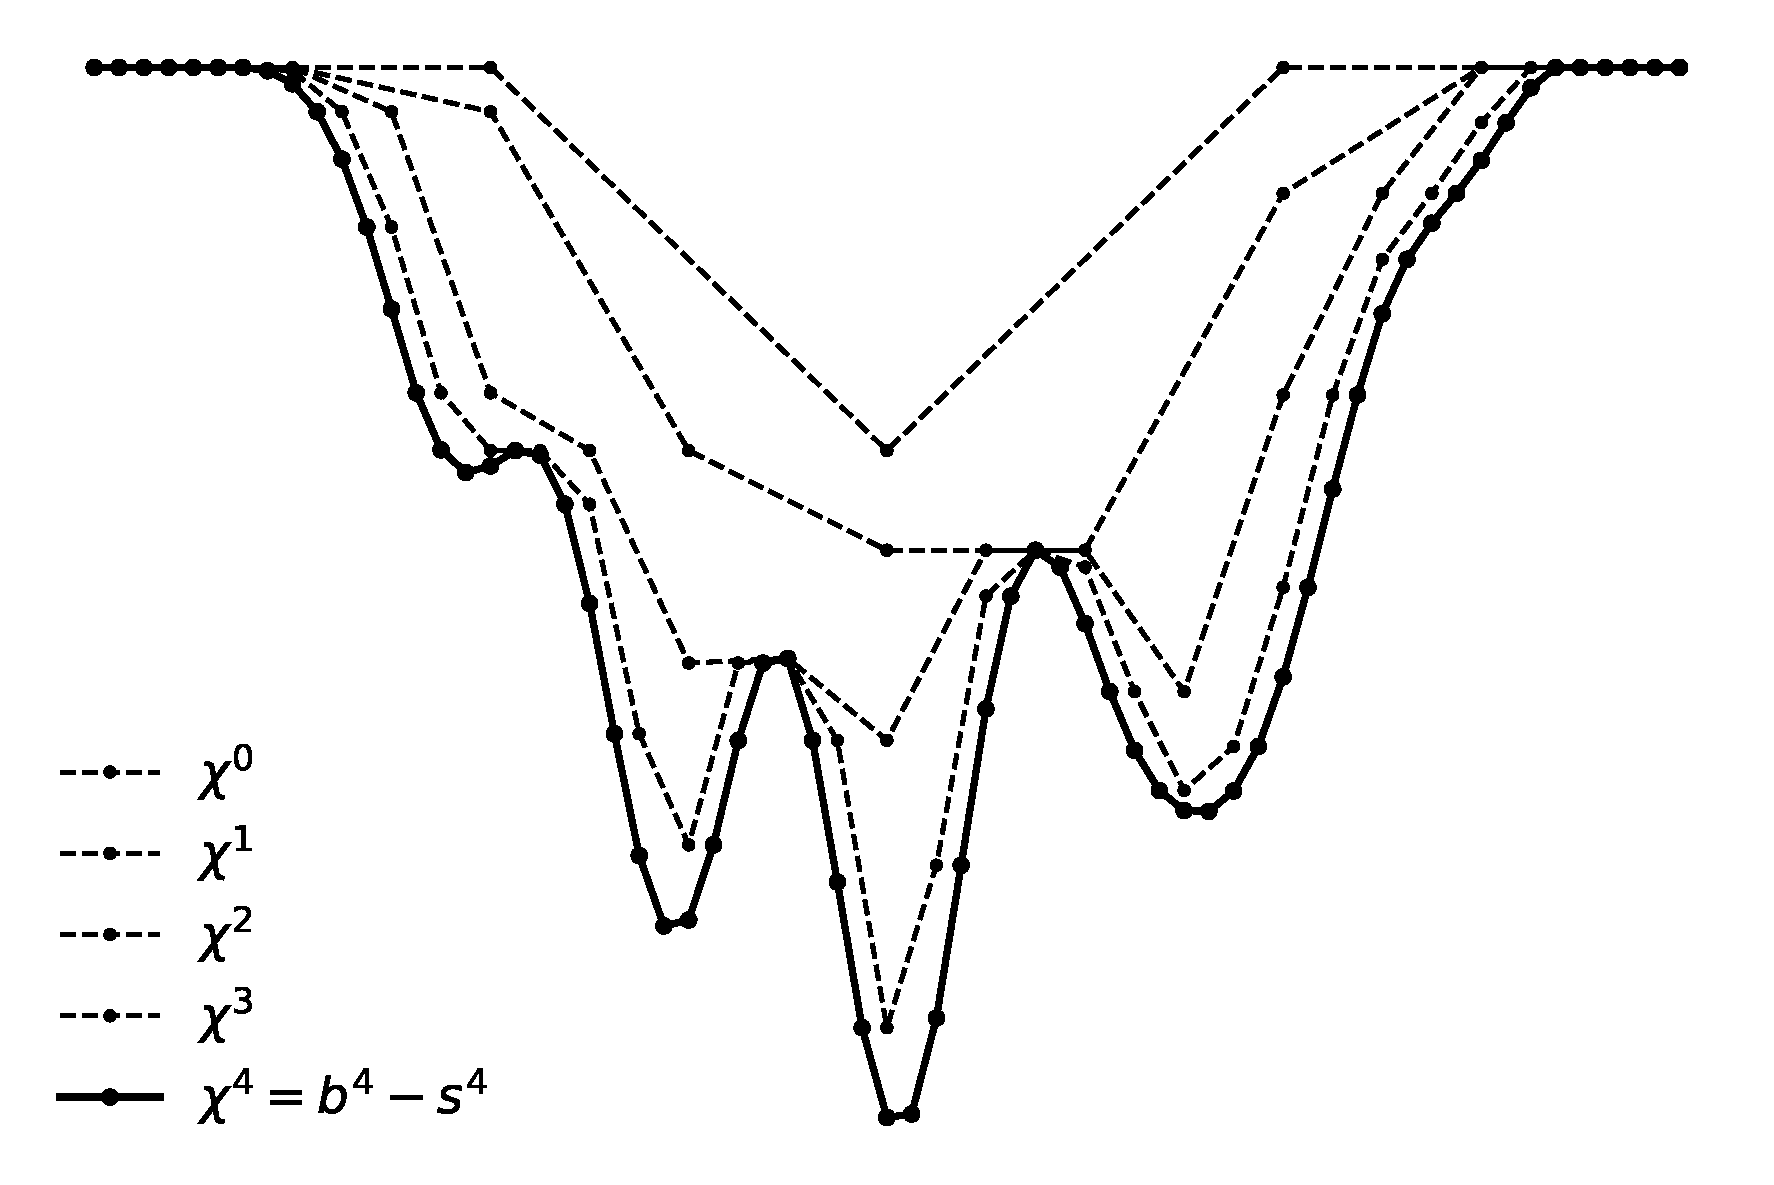
\includegraphics[width=0.7\textwidth]{fixfigs/decompclassical.pdf}
\end{center}
\caption{An example ($d=1$, $J=4$) of an MCD decomposition of the defect obstacle $\chi^J$.  Defect obstacles $\chi^j$ are generated using the monotone restriction operator $\mR$ as in \eqref{eq:recursivedefectobstacle}.}
\label{fig:decompclassical}
\end{figure}

A point-wise smoother on a given level will solve one-dimensional VIs at each node.  However, different admissible sets are used going down and up in the V-cycle.  Let
\begin{equation}
\mathcal{D}^j = \left\{y^j \in \mathcal{V}_0^j \,:\, y^j \ge \phi^j\right\}, \qquad \mathcal{U}^j = \left\{z^j \in \mathcal{V}_0^j \,:\, z^j \ge \chi^j\right\}. \label{eq:downupsets}
\end{equation}
Note that $0 \in \mathcal{D}^j \cap \mathcal{U}^j$; a zero perturbation is always admissible.  The down-admissible constraint sets $\mathcal{D}^j$ sum to an up-admissible constraint set for each level.  The $\mathcal{U}^j$ are themselves nested,
\begin{equation}
\mathcal{U}^0 \subset \mathcal{U}^1 \subset \dots \subset \mathcal{U}^J \subset W_0^{1,\qq}(\Omega). \label{eq:innerconeapprox}
\end{equation}

We seek a solution to VI \eqref{eq:fesigpweakform} on the fine level.  The original idea of Tai \cite{Tai2003} is to use a multilevel constraint decomposition (MCD) like the above  system $\{\mathcal{D}^j\}$ to compute corrections $y^j \in \mathcal{D}^j$ which sum to a solution of the (nonlinear) fine-level VI,
\begin{equation}
F^J(s^J + y^J + \dots + y^j)[v^j - y^j] \ge (a,v^j - y^j) \quad \text{for all } v^j \in \mathcal{D}^j. \label{eq:mcdoriginal}
\end{equation}
(Here $F^J = F^h$ in \eqref{eq:fesigpweakform}.)  Observe that \eqref{eq:mcdoriginal} exploits the simplification $(s^J + y^J + \dots + v^j) - (s^J + y^J + \dots + y^j) = v^j - y^j$.  Also note that $y^J + \dots + y^j \in \mathcal{U}^J$ so the updated fine-level iterate is admissible in the original sense: $s^J + y^J + \dots + y^j \ge b^J$.

In \cite{Tai2003}, VIs \eqref{eq:mcdoriginal} are to be solved on descending levels $j=J$ down to $j=0$, forming a down-slash or V(1,0) cycle.  (See also \cite[Algorithm 4.7]{GraeserKornhuber2009}.)  However, there is no practical way to achieve rapid solution of VI \eqref{eq:mcdoriginal} on coarse levels if the latest iterate $s^J + y^J + \dots + y^j$ must be directly represented; it has fine-level content.  This is the reason to add a full approximation scheme (FAS) \cite{Trottenbergetal2001} coarse-level ``equation'', which is here a nonlinear VI.  In order to implement our approach we will need to state the FAS coarse-level correction equation using appropriate linear restriction and prolongation operators, as follows.

Let $\iR: \mathcal{V}^{j+1} \to \mathcal{V}^j$ be the injection operator \cite{Trottenbergetal2001}.  Suppose $y^j \in \mathcal{D}^j$ denotes the desired down-correction on the $j$th level.  For corrections $y^j \in \mathcal{D}^j$, define $t^j \in \mathcal{V}^j$ as the $j$th-level approximation to the corrected fine-level solution (i.e.~$t^j \approx s^J + y^J + \dots + y^j$),
\begin{equation}
t^j = \begin{cases} s^J, & j=J \\
                    \iR(t^{j+1} + y^{j+1}), & j < J.
      \end{cases}  \label{eq:fassolution}
\end{equation}
Note that $t^j$ satisfies $t^j \ge \iR(\dots(\iR(b^J))\dots)$ by construction because $y^j \in \mathcal{D}^j$.  Though represented on a coarse level, $t^j$ has admissible point values relative to the fine bed $b^J$.

Let $F^j$ represent the FE discretization of $F$ (Section \ref{sec:fe}) on the $j$th level, and let $R: (\mathcal{V}^{j+1})^* \to (\mathcal{V}^j)^*$ be the canonical restriction on functionals \cite{GraeserKornhuber2009}.  The FAS coarse-level VI is
\begin{equation}
F^j(t^j+y^j)[v^j-y^j] \ge \ell^j[v^j-y^j] \quad \text{for all } v^j \in \mathcal{D}^j. \label{eq:fasequation}
\end{equation}
where
\begin{equation}
\ell^j[v] = \begin{cases} \ip{a}{v}, & j=J \\
                          F^j(t^j)[v] + R \left(\ell^{j+1} - F^{j+1}(t^{j+1}+y^{j+1})\right)[v], & j < J. \end{cases}  \label{eq:fasell}
\end{equation}
On the one hand, all quantities in VI \eqref{eq:fasequation} are represented on the $j$th level, without reference to finer-mesh data.  On the other hand, for $j<J$ the VI \eqref{eq:fasequation} can be rearranged using \eqref{eq:fasell} to a correction form like the FAS equation for PDEs (e.g.~\cite[equation (5.3.12)]{Trottenbergetal2001}),
\begin{equation}
F^j(t^j+y^j)[v^j-y^j] - F^j(t^j)[v^j-y^j] \ge R \left(\ell^{j+1} - F^{j+1}(t^{j+1}+y^{j+1})\right)[v^j-y^j], \label{eq:fasequationtraditional}
\end{equation}
for all $v^j \in \mathcal{D}^j$.  In \eqref{eq:fasequationtraditional} the functional on the left and right side should be smooth, thus explaining \eqref{eq:fasequation}.  Following the solution of \eqref{eq:fasequation} on all descending levels $j=J,\dots,0$, in fact done by a smoother on each level, a V(1,0) cycle is completed and the new fine-mesh iterate is $s^J + y^J + \dots + y^0$.

The above formulas suffice for a V(1,0) cycle, and represent the FAS extension of Algorithm 4.7 in \cite{GraeserKornhuber2009}, and of the method of Tai \cite{Tai2003}.  However, for better performance we note that on the ascending part of a V-cycle we can smooth in a less-constrained set, the larger set $\mathcal{U}^j \supset \mathcal{D}^j$.  Regarding admissibility, the difference between descending and ascending in a V-cycle is that in the former case there are yet-to-be-computed corrections which we must force into small-enough sets $\mathcal{D}^j$ so that their sum is still admissible.  When ascending we have already summed the coarser-level corrections so we can smooth the result in the larger, nested sets $\mathcal{U}^j$ without destroying the admissibility of the yet-finer corrections to come.

The above ideas define the following MCDN V-cycle Pseudocode \ref{pc:mcdn-vcycle}.  This algorithm calls a smoothers from Section \ref{sec:smoothers} and it uses the canonical prolongation $P:\mathcal{V}^j \to \mathcal{V}^{j+1}$.  The default settings correspond to a V(0,1) cycle which we have found to be most efficient in tests on the classical obstacle problem \cite{Bueler2022}.  The returned value is a correction to the current iterate $s^J$.

\begin{pcode}[ht]
\begin{pseudo*}
\pr{mcdn-vcycle}(J,s^J,b^J,\id{down}=0,\id{coarse}=1,\id{up}=1)\text{:} \\+
    $\chi^J, \,\ell^J, \,t^J = b^J - s^J, \,\ip{a}{\cdot}, \,s^J$ \\
    for $j=J$ downto $j=1$ \\+
      $\chi^{j-1} = \mR \chi^j$ \\
      $\phi^j = \chi^j - \chi^{j-1}$ \\
      $y^j = 0$ \\
      $\text{\pr{smoother}}^{\text{\id{down}}}(y^j,t^j,\ell^j,\phi^j)$ \qquad \qquad \ct{in $\mathcal{D}^j$} \\
      $t^{j-1} = \iR(t^j + y^j)$ \\
      $\ell^{j-1} = F^{j-1}(t^{j-1}) + R(\ell^j - F^j(t^j+y^j))$ \\-
    $y^0 = 0$ \\
    $\text{\pr{smoother}}^{\text{\id{coarse}}}(y^0,t^0,\ell^0,\chi^0)$ \qquad \qquad \ct{in $\mathcal{U}^0$} \\
    $z^0 = y^0$ \\
    for $j=1$ to $j=J$ \\+
      $z^j = P z^{j-1} + y^{j}$ \\
      $\text{\pr{smoother}}^{\text{\id{up}}}(z^j,t^j,\ell^j,\chi^j)$ \qquad \qquad \ct{in $\mathcal{U}^j$} \\-
    return $z^J$
\end{pseudo*}
\caption{MCDN V-cycle.}
\label{pc:mcdn-vcycle}
\end{pcode}

To our knowledge two aspects of this MCDN V-cycle are new:
\begin{enumerate}
\item While Tai \cite{Tai2003} defines and proves the convergence of a nonlinear MCD method, the implementation of this method cannot achieve $O(m_J)$ time for each V-cycle in nonlinear cases because the method refers to the fine level for the residual evaluation on each coarser level.  Our FAS-type modification achieve $O(m_J)$ time per V-cycle when applied to a local nonlinear problem, for example in the SIA model application in \cite{Bueler2022} in which the smoother is $O(m_j)$ on each level.  In our current Stokes case the smoother is nonlocal and $O(m_j)$ smoother time is not achieved.
\item Our V($\alpha$,$\beta$) cycles, with $\alpha$ down-smoother and $\beta$ up-smoother applications, are more efficient when $\beta >0$ than the method proposed in \cite{GraeserKornhuber2009} for $V(1,1)$ cycles because the smoothing occurs in a less-constrained set.
\end{enumerate}

Finally we consider when iterated V-cycles have converged.  For any discrete obstacle $\chi^j \in \mathcal{V}^j$, admissible iterate $z^j\in \{r^j \ge \chi^j\} \subset \mathcal{V}^j$, and residual vector $r^j \in (\mathcal{V}^j)'$ let
\begin{equation}
\vertiii{r^j}_{(z^j,\chi^j)} = \left(\sum_{z_i > \chi_i} |r^j[\psi_i^j]|^2 + \sum_{z_i = \chi_i} |\min\{r^j[\psi_i^j],0\}|^2\right)^{1/2}, \label{eq:cpnorm}
\end{equation}
where $\psi_i^j$ denotes a $j$th-level nodal basis function.  This defines a ``CP residual norm'' associated to the finite-dimensional complementarity problem $z^j \ge \chi^j$, $r^j(z^j) \ge 0$, and $(z^j-\chi^j) r^j(z^j) = 0$.  Note $z^j \in \mathcal{V}^j$ solves this CP if and only if $z^j$ is admissible and $\vertiii{r^j(z^j)}_{(z^j,\chi^j)}=0$.

As shown in Pseudocode \ref{pc:mcdn-solver}, we iterate MCDN V-cycles until the CP residual norm is small according to either an absolute or a relative tolerance.

\begin{pcode}[ht]
\begin{pseudo*}
\pr{mcdn-solver}(J,s^J,b^J,\id{atol}=10^{-20},\id{rtol}=10^{-3},\id{stol}=10^{-20},\id{max}=100)\text{:} \\+
    $\rho_0=\vertiii{(a,\cdot) - F^J(s^J)[\cdot]}_{(s^J,b^J)}$ \\
    for $k=1,\dots,\id{cyclemax}$ \\+
        $z^J = \pr{mcdn-vcycle}(J,s^J,b^J)$ \\
        $s^J \gets s^J + z^J$ \\
        $\rho_k=\vertiii{(a,\cdot) - F^J(s^J)[\cdot]}_{(s^J,b^J)}$ \\
        if $\rho_k < \id{atol}$ or $\rho_k \le \id{rtol} \, \rho_0$ or $\|z^J\| \le \id{stol}$ \\+
            break \\--
\end{pseudo*}
\caption{The SIGP is solved in-place by iterating V-cycles (Pseudocode \ref{pc:mcdn-vcycle}) until the CP residual norm \eqref{eq:cpnorm} is small.}
\label{pc:mcdn-solver}
\end{pcode}


\section{Performance models} \label{sec:perfmodels}

FIXME


\section{Results for steady geometry} \label{sec:results}

FIXME The computations in this section use the Python FE library Firedrake \cite{Rathgeberetal2016}, which applies an embedded domain language \cite{Alnaesetal2014} to convert weak forms into discrete equations which are solved in parallel using the PETSc \cite{Balayetal2020} library.  Each time the smoother is applied the Glen-Stokes problem is solved, by Newton linearization and (parallel) direct solution of the Newton step equations, in order to evaluate the IDO $\Phi(s)$.  To replace this non-scalable approach we propose in future work to apply existing geometric \cite{BrownSmithAhmadia2013,IsaacStadlerGhattas2015} and algebraic \cite{Tuminaroetal2016} multigrid strategies.

FIXME convergence results; scaling results


\section{Multilevel methods for evolving geometry} \label{sec:evolution}

FIXME time-dependent runs


\section*{Acknowledgments}  Thanks to David Maxwell for discussions regarding the formulation of the model.

\small

\bigskip
\bibliography{msg}
\bibliographystyle{siam}

\appendix

\section{Glossary of acronyms} \label{app:glossary}

\renewcommand{\arraystretch}{1.1}
\begin{longtable}{l|l|l}
\caption{Glossary of acronyms used in this paper.}
\label{tab:acronyms} \\ % \\ REQUIRED HERE
\toprule
\textbf{Acronym} {\Large$\strut$} & \textbf{Definition} & \textbf{Reference} \\ \hline
CMB & climatic mass balance & Section \ref{sec:stokesgeometry} \\
FAS & full approximation scheme & Section \ref{sec:mcdstokes} \\
FE & finite element & Section \ref{sec:fe} \\
GS & Gauss-Seidel & Section \ref{sec:smoothers} \\
IDO & ice dynamics operator & Section \ref{sec:weakido}, equation \eqref{eq:ido} \\
IIGP & implicit ice geometry problem & Section \ref{sec:evolution} \\
MCD & multilevel constraint decomposition & Section \ref{sec:mcdstokes} \\
MCDN & multilevel constraint decomposition (nonlinear) & Section \ref{sec:mcdstokes}, Pseudocode \ref{pc:mcdn-vcycle} \\
NCP & nonlinear complementarity problem & Section \ref{sec:stokesgeometry} \\
PNGS & projected, nonlinear Gauss-Seidel (smoother) & Section \ref{sec:smoothers}, Pseudocode \ref{pc:pngsslow} \\
PNJ & projected, nonlinear Jacobi (smoother) & Section \ref{sec:smoothers}, Pseudocode \ref{pc:pnj} \\
SIA & shallow ice approximation & Section \ref{sec:intro} \\
SIGP & steady ice geometry problem & Section \ref{sec:stokesgeometry}, equation \eqref{eq:strongform} \\
SKE & surface kinematical equation & Section \ref{sec:stokesgeometry}, equation \eqref{eq:ske} \\
VI & variational inequality & Section \ref{sec:weakido} \\
WU & work units & Section \ref{sec:mcdstokes} \\ % final \\ required
\bottomrule
\end{longtable}

\end{document}
